\documentclass{ctexart}
\usepackage{avanti-color}
%\usepackage{avanti-font}
\usepackage{avanti-math}
\usepackage{avanti-theorem}
\usepackage{avanti-others}

\RequirePackage{fontspec}
\xeCJKsetup{CJKmath=true}
\setCJKmainfont[BoldFont=FZHei-B01,ItalicFont=]{LXGW Bright}

\everymath{\color{Solarized-magenta}}
\pagestyle{empty} % 没有页眉和页脚

% define the plot style and the axis style
\tikzset{font=\Large}
\tikzset{base/.style={smooth, thick, Solarized-base01}}
\tikzset{arrow/.style={>=stealth, base}}

\begin{document}

\begin{center}
    \begin{tikzpicture} [scale = 0.8]
        \tikzset{level distance=50pt, sibling distance=0pt}
        \tikzset{edge from parent/.append style={very thick, Solarized-base01}}
        \tikzset{level 4+/.style={level distance=25pt}}
        \tikzset{edge from parent/.style = {draw, thick, Solarized-base01, edge from parent path={(\tikzparentnode.south) -- +(0,-8pt) -| (\tikzchildnode)}}}
        \Tree 
        [.$cn^2$
            [.$c(\frac{n}{4})^2$
                    [.$c(\frac{n}{16})^2$
                            [.$\vdots$ \edge[Solarized-base3]; $\Theta(1)$ ]
                                [.$\vdots$ ]
                                [.$\vdots$ \edge[Solarized-base3]; $\Theta(1)$ ] ]
                        [.$c(\frac{n}{16})^2$
                            [.$\vdots$ ]
                                [.$\vdots$ \edge[Solarized-base3]; $\cdots$ ]
                                [.$\vdots$ ] ]
                        [.$c(\frac{n}{16})^2$
                            [.$\vdots$ \edge[Solarized-base3]; $\Theta(1)$ ]
                                [.$\vdots$ ]
                                [.$\vdots$ \edge[Solarized-base3]; $\Theta(1)$ ] ] ]
                [.$c(\frac{n}{4})^2$
                    [.$c(\frac{n}{16})^2$
                            [.$\vdots$ ]
                                [.$\vdots$ \edge[Solarized-base3]; $\cdots$ ]
                                [.$\vdots$ ] ]
                        [.$c(\frac{n}{16})^2$
                            [.$\vdots$ \edge[Solarized-base3]; $\Theta(1)$ ]
                                [.$\vdots$ ]
                                [.$\vdots$ \edge[Solarized-base3]; $\Theta(1)$ ] ]
                        [.$c(\frac{n}{16})^2$
                            [.$\vdots$ ]
                                [.$\vdots$ \edge[Solarized-base3]; $\cdots$ ]
                                [.$\vdots$ ] ] ]
                [.$c(\frac{n}{4})^2$
                    [.$c(\frac{n}{16})^2$
                            [.$\vdots$ \edge[Solarized-base3]; $\Theta(1)$ ]
                                [.$\vdots$ ]
                                [.$\vdots$ \edge[Solarized-base3]; $\Theta(1)$ ] ]
                        [.$c(\frac{n}{16})^2$
                            [.$\vdots$ ]
                                [.$\vdots$ \edge[Solarized-base3]; $\cdots$ ]
                                [.$\vdots$ ] ]
                        [.$c(\frac{n}{16})^2$
                            [.$\vdots$ \edge[Solarized-base3]; $\Theta(1)$ ]
                                [.$\vdots$ ]
                                [.$\vdots$ \edge[Solarized-base3]; $\Theta(1)$ ] ] ] ]
    \end{tikzpicture}
\end{center}

\end{document}